\documentclass{beamer}

\mode<presentation>

\usetheme{Frankfurt}

\setbeamertemplate{navigation symbols}{}
% \setbeamertemplate{frametitle continuation}[from second][(contd.)]
\setbeamertemplate{frametitle continuation}[from second][]

\title{Some Title}
\subtitle{And Maybe a Subtitle}
\author[Illig \and Orvis \and Segawa \and Spinale]{Peter Illig \and Eli Orvis \and Yukihiko Segawa \and Nick Spinale}
\institute[Carleton]{Carleton College}
\date{February 20\textsuperscript{th}, 2018}

\usepackage[english]{babel}
\usepackage[utf8x]{inputenc}
\usepackage[T1]{fontenc}
\usepackage{amsthm,amssymb,amsmath}
\usepackage{graphicx}
\usepackage{tikz}
\usepackage[normalem]{ulem}

\newcommand{\hcancel}[1]{ % red strikethrough
    \tikz[baseline=(tocancel.base)]{
        \node[inner sep=0pt,outer sep=0pt] (tocancel) {#1};
        \draw[red] (tocancel.south west) -- (tocancel.north east);}}
\newcommand{\hunder}[1]{ % red underline
    \tikz[baseline=(tocancel.base)]{
        \node[inner sep=0pt,outer sep=0pt] (tocancel) {#1};
        \draw[red] (tocancel.south west) -- (tocancel.south east);}}

\newcommand{\N}{\mathbb{N}}
\newcommand{\Z}{\mathbb{Z}}
\newcommand{\Q}{\mathbb{Q}}
\newcommand{\CC}{\mathbb{C}}
\newcommand{\g}{\gamma}
\newcommand{\xg}{x-\gamma}
\newcommand{\pxg}{(x-\gamma)}

\begin{document}

\newtheorem{thm}{Theorem}[section]
\newtheorem{prop}[thm]{Proposition}
\newtheorem{cor}[thm]{Corollary}
\newtheorem{obs}[thm]{Observation}
\newtheorem{defn}[thm]{Definition}
\newtheorem{exmp}[thm]{Example}
\newtheorem{remk}[thm]{Remark}

\maketitle

\begin{frame}
  \frametitle{Contents}
  \tableofcontents
\end{frame}

\section{Introduction}

\begin{frame}
  \frametitle{A Title}
  Contents of the slide
\end{frame}


\section{Simplifying the Problem}

\begin{frame}[allowframebreaks]{Roots of $f^n(x)$}

  % TODO show root tree?

  $f(x) = (x-\gamma)^2+\gamma+m$

  \begin{itemize}
    \item The roots of $f(x)$ are $\gamma\pm\sqrt{-m-\gamma}$
    \item If $\alpha$ is a root of $f^n(x)$, then $\gamma\pm\sqrt{\alpha-m-\gamma}$ are roots of $f^{n+1}(x)$
  \end{itemize}

  \begin{obs}
    For $n>0$, the roots of $f^n(x)$ are, with $n$ radicals:
    $$\gamma\pm\sqrt{-m\pm\sqrt{-m\pm\sqrt{-m\pm\ldots\sqrt{-m-\gamma}}}}$$
  \end{obs}

  \framebreak

  \begin{obs}
    For $n>0$, the roots of $f^n(x)$ are, with $n$ radicals:
    $$\gamma\pm\sqrt{-m\pm\sqrt{-m\pm\sqrt{-m\pm\ldots\sqrt{-m-\gamma}}}}$$
  \end{obs}

  For notational convenience, define $\beta : \Sigma^* \rightarrow \CC$ where
  \begin{align*}
    \beta_{\epsilon} &= -\gamma \\
    \beta_{0s} &= \sqrt{-m+\beta_s} \\ 
    \beta_{1s} &= -\sqrt{-m+\beta_s}
  \end{align*}

  For $n>0$, the roots of $f^n(x)$ are exactly $\{\;\gamma+\beta_s\mid s\in\Sigma^n\;\}$.

\end{frame}


\section{Newly Reducible Third Iterates, Part 1}

\begin{frame}[allowframebreaks]{Newly Reducible Third Iterates Part 1}


Let

  \begin{itemize}
    \item $p_1(x) = a + b (\xg) + c (\xg)^{2} + d(\xg)^{3} + (\xg)^{4}$
    \item $p_2(x) = a - b (\xg) + c (\xg)^{2} - d (\xg)^{3} + (\xg)^{4}$
  \end{itemize}

If $f^3 = p_1(p_2)$, then

\begin{align*}
\gamma + m^{4} + 2 m^{3} + m^{2} + m &= a^2 \\
4 m^{3} + 4 m^{2} &= 2ac - b^2 \\
6 m^{2} + 2 m &= 2a - 2bd + c^2 \\
4 m &= 2c - d^{2}
\end{align*}

\framebreak

Every newly reducible third iterate is a rational point on this surface!

\end{frame}

\begin{frame}
\frametitle{Simplifying the System}

We can simplify this system of equations using linear substitutions and the quadratic formula to get

\begin{align*}
\gamma= & \pm\beta \left(- \frac{3 d^{6}}{16} - \frac{d^{4} m}{2} - \frac{d^{2} m^{2}}{2} - \frac{d^{2} m}{2}\right) \\
& + \frac{17 d^{8}}{64} + \frac{5 m}{4} d^{6} + \frac{11 d^{4}}{4} m^{2} + \frac{7 m}{4} d^{4} + 2 d^{2} m^{3} + 2 d^{2} m^{2} - m
\end{align*}

\pause

Note that every expression in this formula is a rational function of $d$, $m$, and $\beta$

\end{frame}

\begin{frame}
\frametitle{All about $\beta$}

Let's look at $\beta$

\begin{equation*}
\beta = \sqrt{2 d^{4} + 8 d^{2} m + 16 m^{2} + 16 m}
\end{equation*}

\pause 

Letting $\beta = y$ and $d = s$ we have the surface

\begin{equation*}
S:\ y^2 = 2 s^4 + 8 m s^2 + 16 m^2 + 16 m
\end{equation*}

\end{frame}

\begin{frame}
\frametitle{The Curves $C_m$}

We want to explore the surface $S$, by considering the curve $C_m$ that results from a fixed value of $m$.

\pause

\begin{equation*}
C_{m_0}:\ y^2 = 2 s^4 + 8 s^2 (m_0) + 16 (m_0)^2 + 16 m_0
\end{equation*}

\pause

Some questions to consider:

\begin{itemize}
\item What are the roots of $C_m$?
\pause
\item What is the genus of $C_m$?
\pause
\item Does $C_m$ have rational points?  If so, how many?
\end{itemize}

\end{frame}

\begin{frame}
\frametitle{The roots of $C_m$}

What do the roots of $C_m$ tell us?

\pause

If $C_m$ has repeated roots, it's a conic!  Otherwise, it's an elliptic curve.

\pause

So when does $C_m$ have repeated roots?

\end{frame}

\begin{frame}
\frametitle{The roots of $C_m$}

\begin{align*}
C_{m_0}:\ y^2 & = 2 s^4 + 8 s^2 (m_0) + 16 (m_0)^2 + 16 m_0 \\
\pause
& = 2(s^2)^2 + 8 s^2 (m_0) + 16 (m_0)^2 + 16 m_0
\end{align*}

\pause

Using the quadratic formula we get that $C_m$ has a repeated root if and only $\sqrt{-2m-m^2} = 0$ or $2(-m\pm\sqrt{-2m-m^2}) = 0$.  This happens when $m \in \{0, -1, -2\}$.


\end{frame}

\end

\end{frame}

\section{Newly Reducible Third Iterates, Part 2}

\begin{frame}[allowframebreaks]
  \frametitle{A New Perspective}
  $$S:y^2 = 2s^4 + 8ms^2 + 16m^2 + 16m$$
  \phantom{hi}
  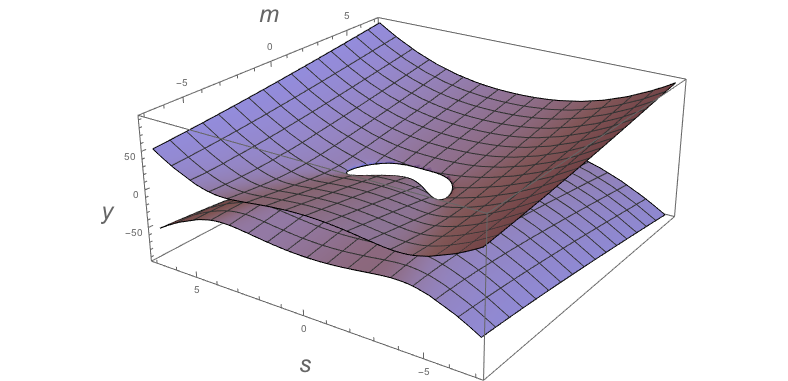
\includegraphics[width=\textwidth]{SPlot.png}
  
\framebreak
  
  So far,
	$$S:y^2 = 2s^4 + 8ms^2 + 16m^2 + 16m$$
	\phantom{hi}
	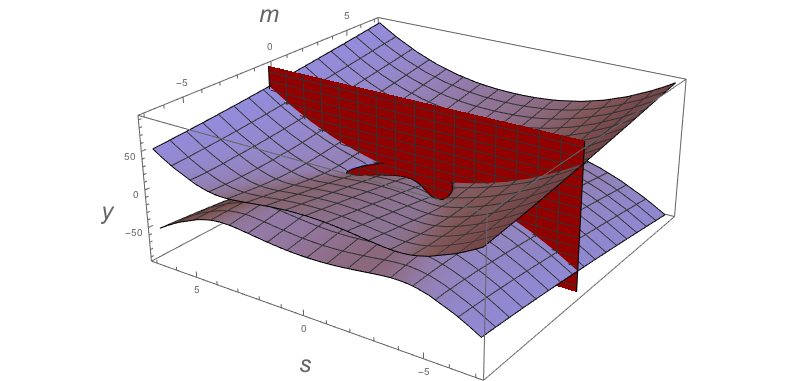
\includegraphics[width=\textwidth]{ECPlot.png}

\framebreak

	$$S:y^2 = 16m^2 + (16+8s^2)m + 2s^4$$
	\phantom{hi}
	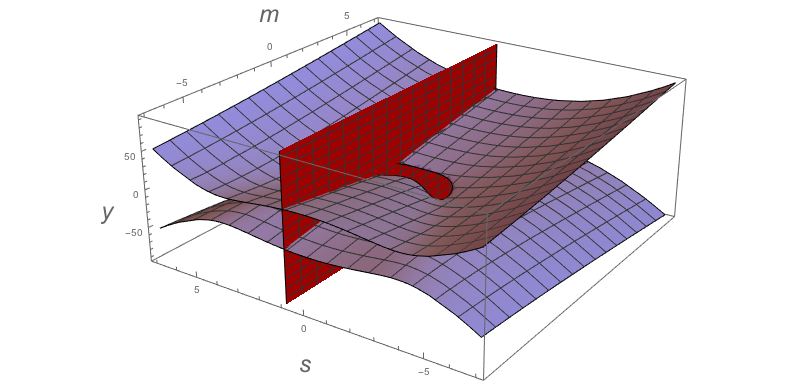
\includegraphics[width=\textwidth]{CSPlot.png}
	
	\framebreak
	
	This is a conic! $$y^2 = am^2 + bm + c$$
	\phantom{hi}
	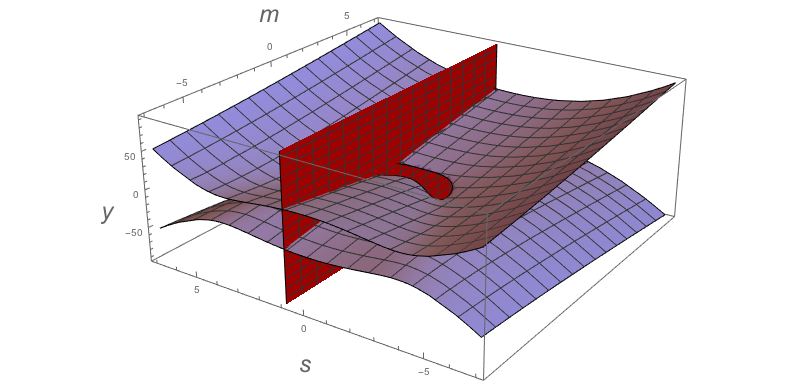
\includegraphics[width=\textwidth]{CSPlot.png}
\end{frame}

\begin{frame}
	\frametitle{Rational Projection}
	For any $s$, we have
	$$y^2 = 16m^2 + (16+8s^2)m + 2s^4.$$
	\pause
	To use projection, we need a point on this curve.\\
	\pause
	Luckily, we can use the point at infinity!
\end{frame}
	
\begin{frame}
	\frametitle{Rational Projection}
	$$S: y^2 = 16m^2 + (16+8s^2)m + 2s^4$$
	\pause
	\begin{obs}
		We're only looking for \textbf{rational} solutions.
	\end{obs}
	\pause
	$$\mbox{Let }y = \frac{Y}{Z}\mbox{ and }m = \frac{M}{Z}.$$
	\pause
	\begin{defn}
		The \textbf{homogeneous form} of $S$ is
		$$S: Y^2 = 16 M^2 + (8 s^2 + 16) M Z + 2 s^4 Z^2.$$
	\end{defn}
\end{frame}

\begin{frame}
	\frametitle{Rational Projection}
	If $Z=0$...
	\pause
	$$Y^2 = 16 M^2 + (8 s^2 + 16) M Z + 2 s^4 Z^2$$
	\pause
	$$Y^2 = 16 M^2 +\text{ \hcancel{\ensuremath{(8 s^2 + 16) M Z}}} + \text{ \hcancel{\ensuremath{2 s^4 Z^2}}}$$
	\pause
	$$ Y^2 = 16 M^2 $$
	\pause
	$$ Y=\pm 4 M$$
\end{frame}

\begin{frame}
	\frametitle{Rational Projection}
	\begin{obs}
		The point $[M:Y:Z]=[1:4:0]$ is a solution to the homogeneous form of $S$.
	\end{obs}
	\pause
	\begin{center}
		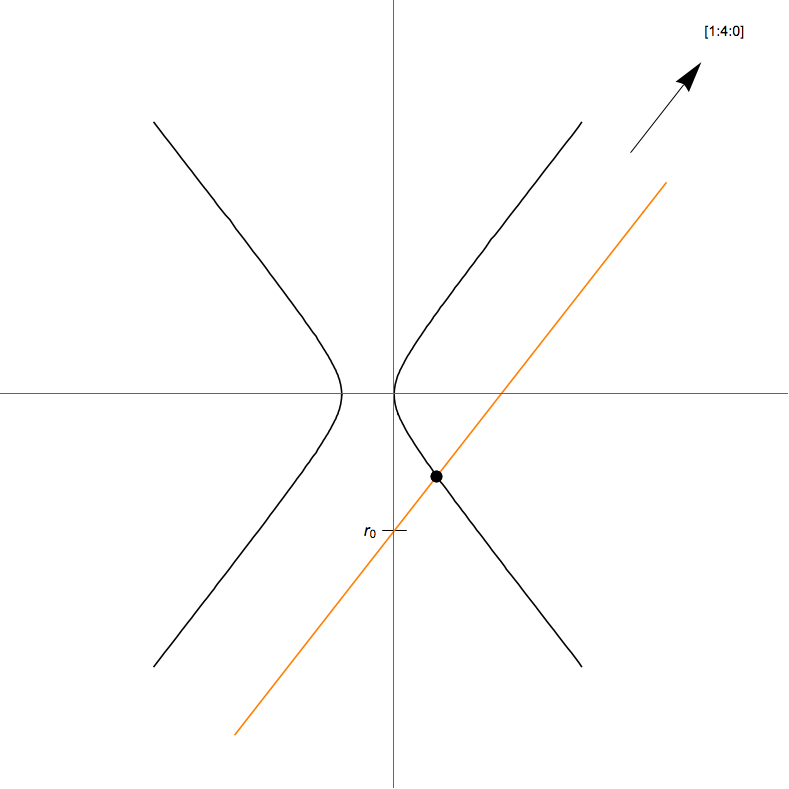
\includegraphics[width=.5\textwidth]{projection-from-infinity.png}
	\end{center}
\end{frame}





























\end{document}




